\subsubsection{الگوی \lr{Microkernel}}
\label{archMicrokernelSec}
\begin{RTL}
الگوی معماری میکروکرنل \cite{ref4} برای سیستم‌هایی که دارای مجموعه‌ای اصلی
از خدمات هستند که می‌توانند در زمان ساخت با خدمات
اضافی گسترش یابند، مفید است.
این الگو با ارائه قابلیت پیکربندی در زمان ساخت،
قابلیت استفاده مجدد و تنظیم‌پذیری را افزایش می‌دهد و به توسعه‌دهندگان اجازه
می‌دهد تا خدمات مورد نیاز برای یک برنامه را انتخاب
کنند. یک مثال معمولی، سیستم‌عامل بی‌درنگ
است که دارای خدمات اصلی مانند مدیریت وظایف
و تخصیص حافظه است و می‌تواند با مؤلفه‌های ارتباطات،
خدمات فایل، شبکه و میان‌افزار گسترش یابد.
این الگو از مقیاس‌پذیری و تطبیق‌پذیری در
طیف گسترده‌ای از برنامه‌ها، از سیستم‌های کوچک با محدودیت
حافظه تا سیستم‌های پیچیده و شبکه‌ای، پشتیبانی می‌کند.
\end{RTL}
\begin{figure}[h!]
\centering
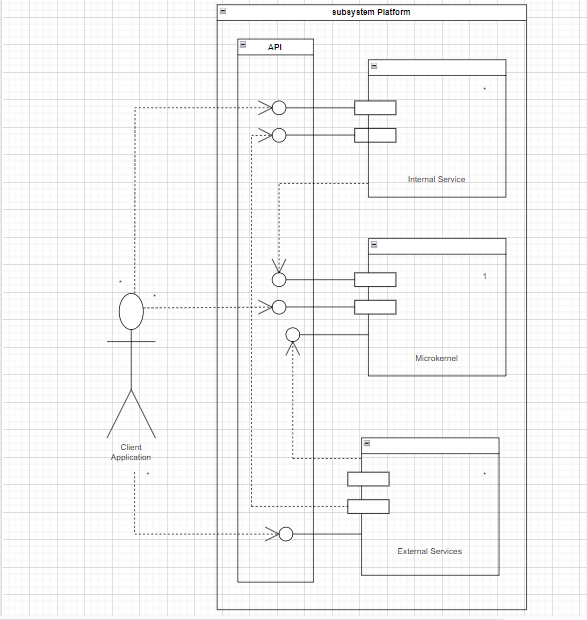
\includegraphics[scale=0.5]{images/first/microkernel.png}
\caption{ساختار الگوی \lr{Microkernel}}
\end{figure}